% ここはもともとパラメーターのための予備実験を書くところだった
% どうするかはあなたに一任するわ
\chapter{実装と予備実験}
ここでは本研究を行うにあたり実装したシステムと予備実験および、その改善について述べる。
%\subsection{データセット}
%この研究ではドライブレコーダーから得られる映像を用いて実験を行う.
%その際,データーセットとしてYouTube等の動画投稿サイトに投稿されたドライブレコーダーの動画を用いる.
\section{予備実験1 - 深度推定システム}
\subsection{実験内容}
本研究ではドライブレコーダーから得られる動画を用いて実験,評価を行うが,その予備実験として動画から切り出された画像を用いて本研究のシステムの実験を行った.
この予備実験は,本研究を行うにあたって,距離推定プログラムあるいは深度推定プログラムの候補が2つあり,どちらが相応しいかを決める実験である.
一つ目はFCRN-DepthPrediction\cite{laina2016deeper}というシステムであり,もう一つはstruct2depth\cite{casser2019struct2depth}である.
元の画像および2つの深度推定ライブラリを使用した結果を\figref{fig:depth_raw},\figref{fig:preex}および\figref{fig:preex2}に示す.
\figref{fig:preex}のように,このシステムは画像を上下二段に切り分け,上段では入力された映像の高さを半分にした画像,下段はその画像を用いて奥行き推定を行ったものである.
また,上段で自動車とトラックを検出し,下段の同じ位置にBBOXを出力している.
下段のBBOX内に出力されているパラメーターは,下段BOX内のRGB値のそれぞれの値を平均した数値である.
\newpage
% --------------------------------------------

\begin{figure}[htbp]
  \begin{center}
    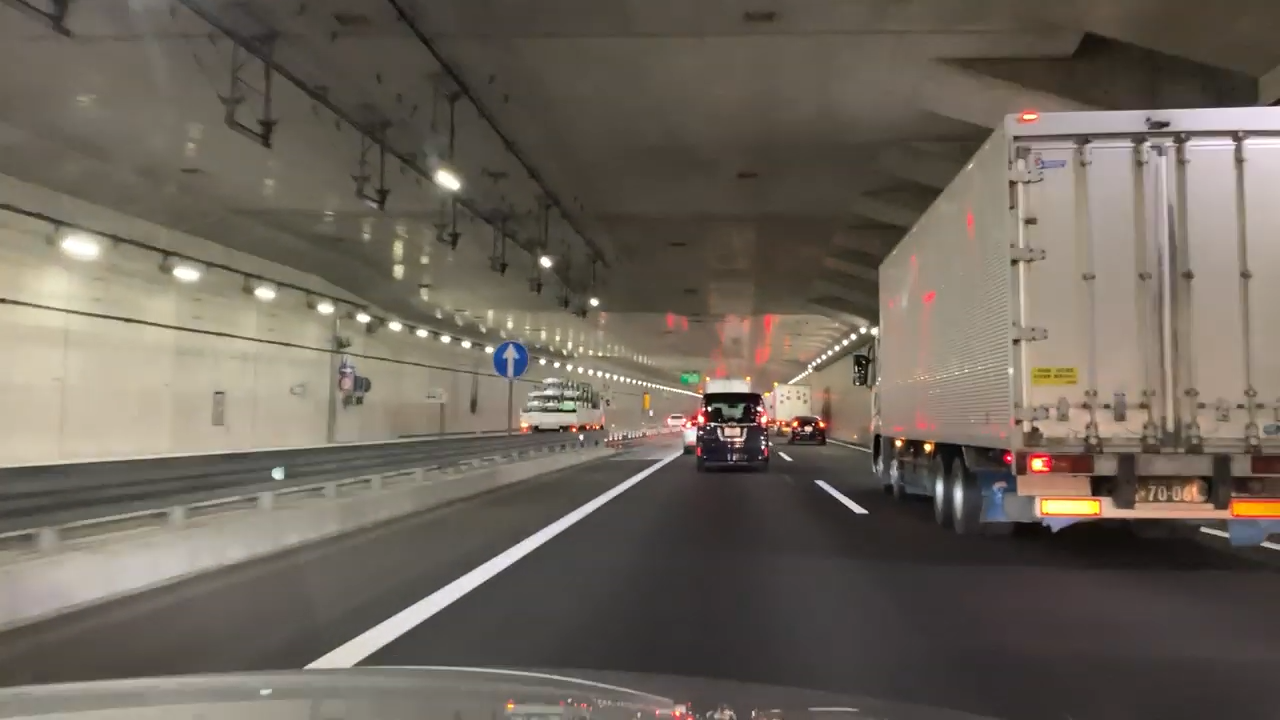
\includegraphics[width=12cm]{figs/depth_raw.png}
   \end{center}
   \caption{元の画像データー}
   \label{fig:depth_raw}
  \end{figure}

  \begin{figure}[htbp]
  \begin{center}
   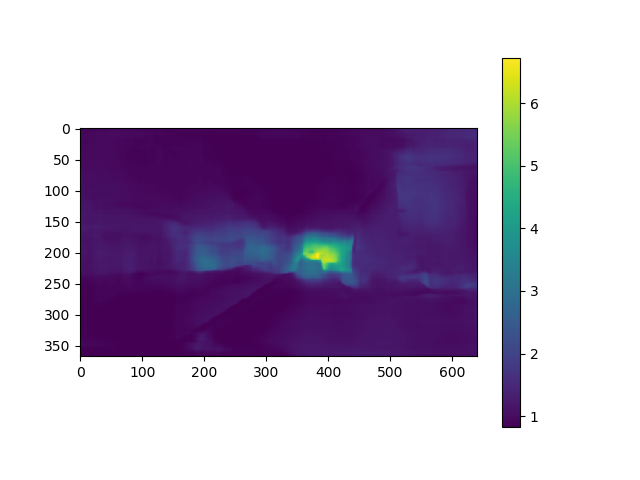
\includegraphics[width=12cm]{figs/preex1.png}
  \end{center}
  \caption{FCRN-DepthPredictionを用いたもの}
  \label{fig:preex1}
\end{figure}

\begin{figure}[htbp]
 \begin{center}
  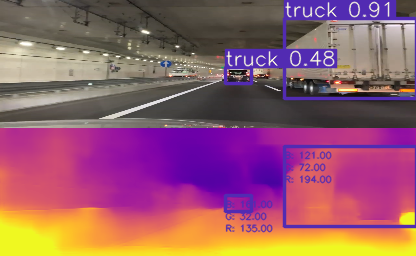
\includegraphics[width=12cm]{figs/preex2.png}
\end{center}
  \caption{struct2depthを用いたもの}
  \label{fig:preex2}
\end{figure}
% ----------------------------------------------
\newpage
\subsection{評価}
ここでは,本研究における予備実験の評価について述べる.
\figref{fig:preex1}と\figref{fig:preex2}を比較すると,前者は深度推定を行なった結果のみを出力するのに対し,後者は元の画像を圧縮し上下二段二分けて出力されていることがわかる.
また,前者は奥にある物体が明るく色分けされているが,カメラから近いところにある道路やトラックなど,ほぼ暗い青色で塗り分けられているだけであり,物体の識別が難しい.
それに対して後者はカメラから近い距離にある物体ほど明るく塗り分けられており,奥にある物体ほど暗い色になっている.
前者と後者を比較した際,特に違いが顕著なのは後者のシステムの方が画面左側にあるトラックをはっきりと色分けできているという点である.
滋養の実験を踏まえて,本研究においては後者のGoogle Tensorflowを採用し,本実験を行うことにする.

また,\figref{fig:preex2}を見ればわかる通り,物体検出システムと距離推定システムを用いることで先行車との大まかな車間距離を調べることが可能なことがわかる.
\figref{fig:preex2}においてシステムが検出した自動車をそれぞれ右から車1,車2とおくと,下段のRGB値のそれぞれの平均を見てみると,奥にある車1の方が手前にある車2よりもR,Gの値が低く,Bの値が高いことがわかる.
%距離推定システムは奥行きを手前にある物体ほど色を明るく,奥にある(カメラから距離が遠い)物体ほど暗い青色で色分けするので,このシステムで先行車の位置関係が大まかにわかることが確認できる.
この数値の違いを評価することで先行車との距離を推定し,走行スピードを推定し,渋滞しているかどうかを機械に判断させる.


% 動画への適用 ---------------------------------
% 画像処理の話
\newpage
\section{予備実験2 - 動画への適用}
ここでは2つめに行った予備実験について述べる.
\subsection{実験内容}
この予備実験は,予備実験1にて行ったシステムを動画へ適用する際に行った実験である.
予備実験1では使用した二つのライブラリ(物体検出ライブラリと深度推定ライブラリ)はどちらも画像のデーターを中間ファイルを通して処理していた.
しかし,動画を使った画像処理をこなうためには,中間ファイルを経由しての処理は余分な処理を増やしてしまい,処理量と処理時間がかかってしまう問題がある.
そのため,今後は中間ファイルを経由することなくデータをやり取りするように実行した.
その際に,深度推定ライブラリ(struct2depth)に合わせて画像サイズを416 * 128の高さの半分である 416 * 64サイズに圧縮して処理するよう実装した.
しかし,画像サイズが圧縮されたため,物体検出ライブラリでの誤検出や検出できないといった問題が起きた.

\subsection{症例}
画像を圧縮してから検出を行った際に起きたミスとしては2つあり,それぞれ誤検出と検出できないという症例である.
その検出結果を\figref{fig:miss1}と\figref{fig:miss2}に示す.

% --------------------------------------------------
\newpage
\begin{figure}[htbp]
  \begin{center}
   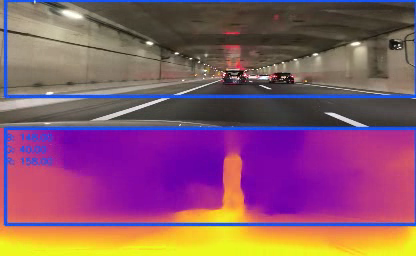
\includegraphics[width=12cm]{figs/miss_1.png}
  \end{center}
  \caption{症例1 - 誤った検出}
  \label{fig:miss1}
\end{figure}

\begin{figure}[hbtp]
 \begin{center}
  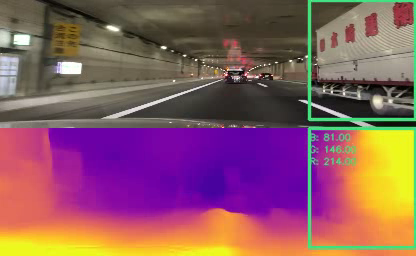
\includegraphics[width=12cm]{figs/miss_2.png}
 \end{center}
  \caption{症例2 - 自動車を検出できなかった症例}
  \label{fig:miss2}
\end{figure}

\newpage
% ---------------------------------------------------

\subsection{解決アプローチ}
症例の原因は元の深度推定ライブラリに合わせて画像を圧縮したため,物体検出システムがうまく機能しなかったためだと考えられる.
問題の解決のため,画像圧縮を避けて画像サイズを416 * 256のまま処理できるように改良した.
その結果,症例で見られるような誤検出や自動車を検出できないといった症例はほとんど見られなくなった.
また,信号機や建物等,渋滞の推定のために必要のない物体を検出しないように,検出物体を自動車類(車,バス,トラック)に絞った.
その実装したプログラムを同じ画像フレームを用いて実験した結果を以下に示す.

% --------------------------------------------------
\begin{figure}[htbp]
  \begin{minipage}{0.5\hsize}
   \begin{center}
    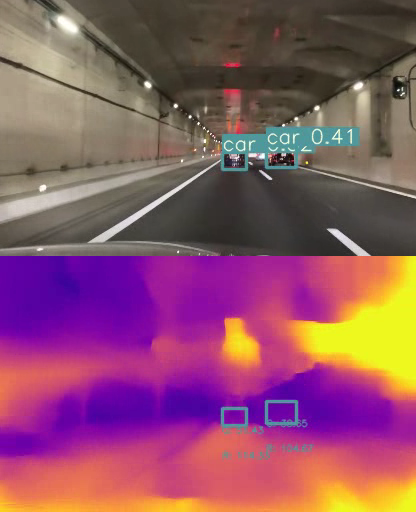
\includegraphics[width=7cm]{figs/pre1_after.png}
   \end{center}
   \caption{症例1の解決}
   \label{fig:pre2after1}
  \end{minipage}
  \begin{minipage}{0.5\hsize}
  \begin{center}
   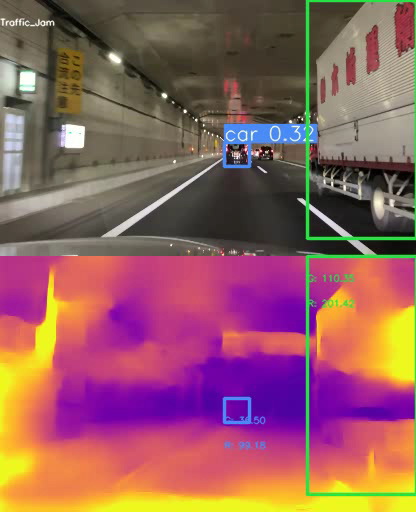
\includegraphics[width=7cm]{figs/pre1_after2.png}
  \end{center}
   \caption{症例2の解決}
   \label{fig:pre2after2}
  \end{minipage}
 \end{figure}

% ---------------------------------------------------
\figref{fig:miss1}と\figref{pre2after1},および\figref{fig:miss2}と\figref{pre2after2}を比較すると,画像の圧縮を抑えた分,誤検出や検出できていない問題が大幅に改善できていることがわかる.
この予備実験2の結果を踏まえて,今後使用する映像圧縮サイズは416 * 256サイズとし,最終的に出力されるサイズはstrct2depthのデーターを加えた416 * 512サイズとする.

\newpage
\section{予備実験3 - 評価方法の決定}
ここでは3つめに行った予備実験について述べる.
\subsection{実験内容}
この予備実験は,本研究における渋滞の評価の基準を決める実験である.
本研究にて使用する深度推定システム(struct2depth)\cite{casser2019struct2depth}は奥行きを推定するシステムだが,\figref{fig:preex2}の通り,結果は色情報でしかわからず,具体的にカメラからどれだけの距離があるのかが不明である.
そのためこの予備実験2では渋滞評価のために出力された色データーから渋滞の基準を決める実験を行う.
本研究では渋滞を車間距離を利用して推定する手法をとっているため,車間距離によって車のスピードや渋滞がどのように変化するかを参考にする.
基本的に車間距離と速度の関係は一般道と高速道路で異なる.
高速道路においては警視庁指示要項によると走行中の車間距離は「速度の2乗/100」をおおよその安全追随距離としている\cite{highway}.
この場合,時速80kmで走っている場合,安全な車間距離は64mとなる.
これに対して高速道路において渋滞している場合の速度は,渋滞の定義を参照すると安全な車間距離は最大で16mとなっている.
しかし,一般道での車間距離は異なる.信号待ち等での停車中の車間距離はトヨタのwebサイトによるとおよそ車一台分,4〜5mとされている\cite{toyota_web}.
よってこの予備実験においては実際に車間距離が4m,5m,6mの時にstruct2depthにおける値がどのように変化するかを調べ,評価基準を決める.


\subsection{使用するデーター}
ここでは予備実験2にて扱うデーターについて述べる.
この予備実験においては実際に車間距離を4m, 5m, 6mのそれぞれにおいて運転席から撮影した映像を利用する.
その際,自動車のフロントガラスにおいて様々な場所から撮影した.以下にサンプルを示す.

% --------------------------------------------------

\begin{figure}[htbp]
  \begin{tabular}{c}
    \begin{minipage}{0.33\hsize}
      \begin{center}
   \includegraphics[width=4.5cm]{figs/sumple/4m_01.png}
    \end{center}
  \caption{車間距離4m}
  \label{fig:sumple4}
\end{minipage}

  \begin{minipage}{0.33\hsize}
  \begin{center}
    \includegraphics[width=4.5cm]{figs/sumple/5m_02.png}
  \end{center}
  \caption{車間距離5m}
  \label{fig:sumple5}
\end{minipage}

  \begin{minipage}{0.33\hsize}
  \begin{center}
    \includegraphics[width=4.5cm]{figs/sumple/6m_01.png}
  \end{center}
  \caption{車間距離6m}
  \label{fig:sumple6}
\end{minipage}
\end{tabular}
\end{figure}

% ---------------------------------------------------
\subsection{実験方法}
ここでは予備実験3で行った実験方法について述べる.
上記の項で示したサンプルデーターをstruct2depth及びYoloシステムを利用して,それぞれの距離においてstrct2depthの数値がどのように変わるかを調べた.
その際,OpenCVの色情報取得システムを利用し,また検出されたBOXの中においてRGB値それぞれの最大値と平均値を比較しどちらを利用すると良いかについても調べた.
その結果の一部を以下に示す.

% ------------------------------------------------------------

\begin{figure}[htbp]
  \begin{tabular}{c}
    \begin{minipage}{0.33\hsize}
      \begin{center}
   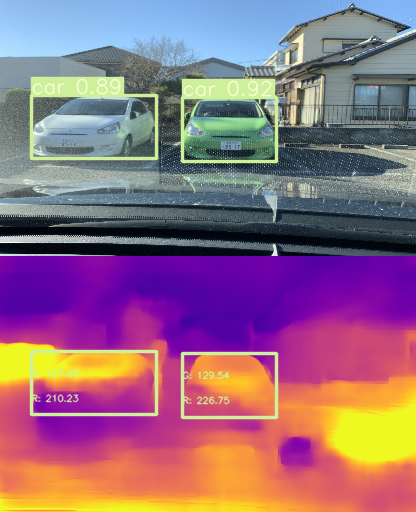
\includegraphics[width=4.5cm]{figs/sumple/4m_02mean.png}
    \end{center}
  \caption{車間距離4m時の平均値}
  \label{fig:sumple4mean}
\end{minipage}

  \begin{minipage}{0.33\hsize}
  \begin{center}
    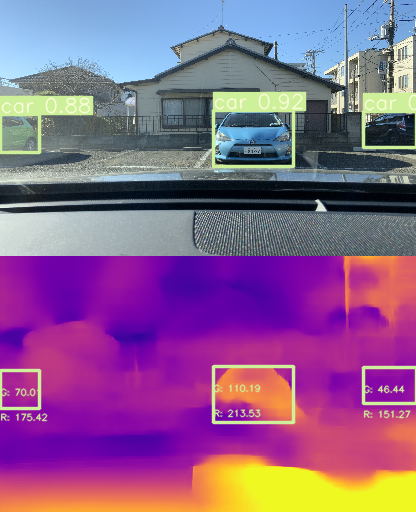
\includegraphics[width=4.5cm]{figs/sumple/5m_02mean.png}
  \end{center}
  \caption{車間距離5m時の平均値}
  \label{fig:sumple5mean}
\end{minipage}

  \begin{minipage}{0.33\hsize}
  \begin{center}
    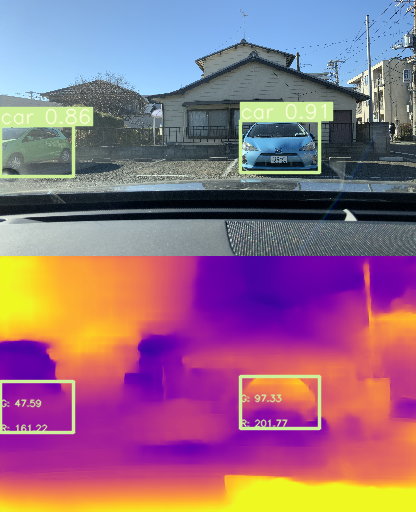
\includegraphics[width=4.5cm]{figs/sumple/6m_01mean.png}
  \end{center}
  \caption{車間距離6m時の平均値}
  \label{fig:sumple6mean}
\end{minipage}
\end{tabular}
\end{figure}

% ------------------------------------------------------------

\begin{figure}[htbp]
  \begin{tabular}{c}
    \begin{minipage}{0.33\hsize}
      \begin{center}
   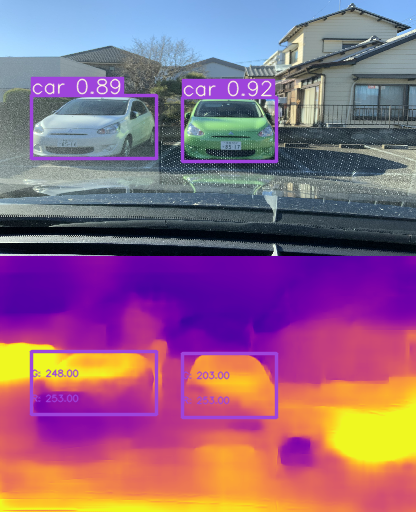
\includegraphics[width=4.5cm]{figs/sumple/4m_02max.png}
    \end{center}
  \caption{車間距離4m時の最大値}
  \label{fig:sumple4max}
\end{minipage}

  \begin{minipage}{0.33\hsize}
  \begin{center}
    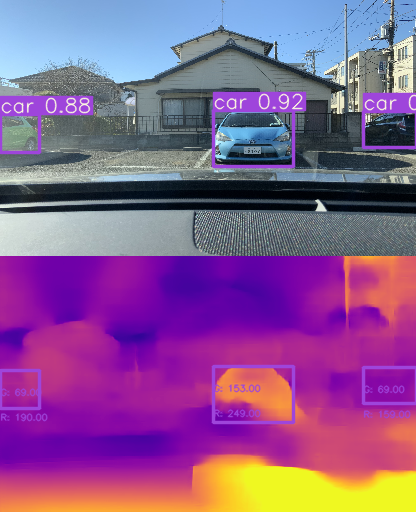
\includegraphics[width=4.5cm]{figs/sumple/5m_02max.png}
  \end{center}
  \caption{車間距離5m時の最大値}
  \label{fig:sumple5max}
\end{minipage}

  \begin{minipage}{0.33\hsize}
  \begin{center}
    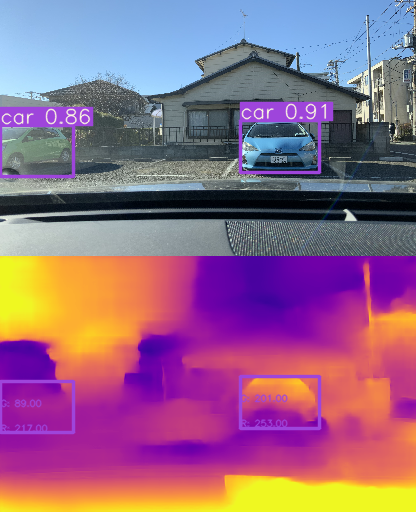
\includegraphics[width=4.5cm]{figs/sumple/6m_01max.png}
  \end{center}
  \caption{車間距離6m時の最大値}
  \label{fig:sumple6max}
\end{minipage}
\end{tabular}
\end{figure}

% ---------------------------------------------------

また,画像の中のR値とG値を改めて以下に表にまとめる.その際,まとめる数値は画面中央に近い自動車の検出された値とする.

% ----------------------------------------------------
\begin{table}[htbp]
  \centering
  \begin{scriptsize}
  \begin{tabular}{ccccccc}
  \toprule
& & 平均値 & 最大値 & & 平均値 & 最大値 \\
  \midrule
4m & R値 & 226.75 & 253.00 & G値 & {\bf129.54} & 203.00 \\
5m & R値 & 213.53 & 249.00 & G値 & {\bf 110.19} & 153.00 \\
6m & R値 & 201.77 & 253.00 & G値 & {\bf 97.33} & 201.00\\
  \bottomrule
  \end{tabular}
  \end{scriptsize}
  \caption{距離別の平均値と最大値}
  \label{tab:mean_max}
\end{table}
% ------------------------------------------------------

\subsection{評価基準の作成}
\tabref{tab:mean_max}からわかることはR値は平均値と最大値のどちらにおいても距離との相関関係は薄いが,G値の特に平均値は距離が近くなるにつれて値が大きくなる傾向があるということである.
この実験結果をもとに,今後の実験においてはG値の平均値を用い,また予備実験3の実験内容の項で述べた通り,車間距離5mを基準とし,G値が100を下回った際に渋滞していると判断する.

\section{ドライブレコーダー映像を用いた予備実験}
\subsection{実験内容}
作成された評価基準を用いて実際にドライブレコーダーにおいてどのようなパフォーマンスをするかの実験を行った。
評価基準の通り、strct2depth画面における車のbbox内のG値が100を超えた際に渋滞と判断し,画面左上に「Traffic Jam」という文字列が表示されるようにした.
加えて,映像中に渋滞が判断された回数をフレームごとにJam Counterとして回数を映像中段左に表示されるようにした.

\subsection{使用したデータセット}
本実験にて使用したデータセットは動画投稿サイトYouTubeにて公開されていた高速道路を走行中の映像に加え,私の家族が使用している自家用車に取り付けられたドライブレコーダー映像を用いる.
どの映像も30秒から1分のものであり,常に先行車がある映像を使用した.以下に使用した映像について表で示す.

% ----------------------------------------------------
\begin{table}[htbp]
  \centering
  \begin{scriptsize}
  \begin{tabular}{ccccc}
  \toprule
映像番号 & 時間帯 & 撮影場所 & 車線数 & 動画時間\\
  \midrule
映像1 & 昼間 & 一般道 & 1 & 60秒\\
映像2 & 昼間 & 一般道 & 2 & 60秒\\
映像3 & 不明 & 高速道路(トンネル) & 2 & 60秒 \\
  \bottomrule
  \end{tabular}
  \end{scriptsize}
  \caption{使用したデータセット}
  \label{tab:dataset}
\end{table}
% ------------------------------------------------------

% 実験1で発生した問題を述べる
\section{実験結果と課題}
実験結果1〜3に
予備実験にて改良したシステムをそのまま用いると,様々な状況で渋滞を誤検出するという問題が発生してしまう.

% --------------------------------------------------
\begin{figure}[htbp]
  \begin{tabular}{c}
    \begin{minipage}{0.33\hsize}
      \begin{center}
   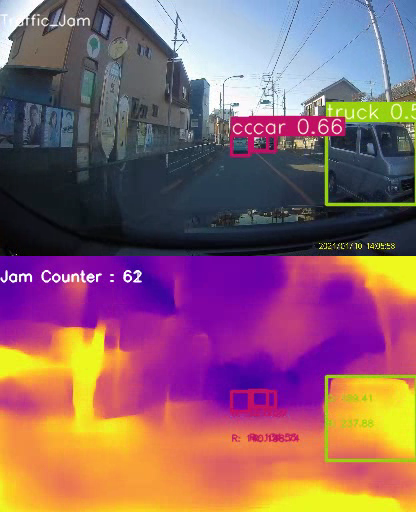
\includegraphics[width=4.5cm]{figs/ex01_01.png}
    \end{center}
  \caption{結果1}
  \label{fig:ex01_01}
\end{minipage}

  \begin{minipage}{0.33\hsize}
  \begin{center}
    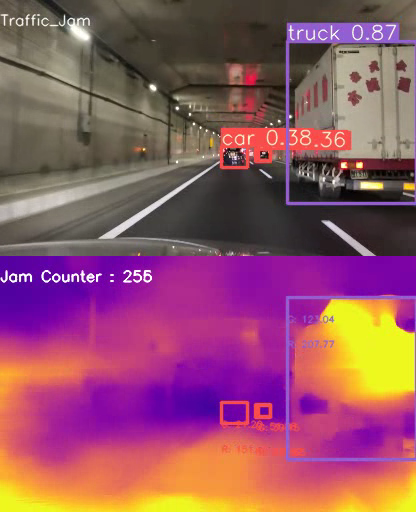
\includegraphics[width=4.5cm]{figs/ex01_02.png}
  \end{center}
  \caption{結果2}
  \label{fig:ex01_02}
\end{minipage}

  \begin{minipage}{0.33\hsize}
  \begin{center}
    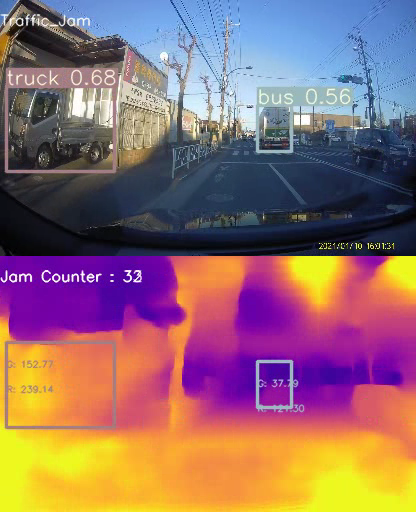
\includegraphics[width=4.5cm]{figs/ex01_03.png}
  \end{center}
  \caption{結果3}
  \label{fig:ex01_03}
\end{minipage}
\end{tabular}
\end{figure}
% ---------------------------------------------------

\figref{fig:ex01_01},\figref{fig:ex01_02},および\figref{fig:ex01_03}の結果からわかるように様々な要因で渋滞の誤検出が起きた.
まず,\figref{fig:ex01_01}においては対向車がドライブレコーダー付きの自動車を横切ってしまうとその際に渋滞と判断してしまう例である.
対向車の存在は渋滞と関係ないのに対し,渋滞と判断してしまうのは正しい判断ではない.
次に,\figref{fig:ex01_02}においては,複数車線がある場合に隣の車線の自動車が近くで走行している際に渋滞だと判断してしいる例である.
先述の対向車のケースとは異なり,隣の車線の混雑は走行車線の混雑と関係がある.
しかし,\figref{fig:ex01_02}のように,先行車との距離があるにもかかわらずたまたま隣で走っていたトラックが近いがために渋滞だと判断してしまうのは正しい判断ではない.
そして,\figref{fig:ex01_03}においては,道路脇に駐車しているトラックを画像検知システムが検知してしまい,渋滞だと判断している例である.
高速道路では稀であるが一般道を走行している際に道路脇に自動車が駐車されているのは珍しいことではなく,またその駐車は渋滞には一切関係がない.
それにもかかわらず渋滞だと判断しているのは正しい判断ではない.
これらの判断ミスのケースは\tabref{tab:dataset}の表にある映像のいずれにおいても頻繁に発生する問題であった.

\subsection{解決アプローチ}
実験1における問題の解決のために対向車,隣車線の自動車および駐車している自動車を検出しないという解決策を取った.
対向車や隣車線の自動車といったものはドライブレコーダー映像において左右の1/3に写っている.
ここに着目し,左右1/3に写っている自動車類の検出をしないように改良した.

\newpage

\section{改良したシステムを用いた実験}
実験1における解決アプローチを元にプログラムを改良した.
プログラムにおいて処理中の画像の横のサイズは416ピクセルなので,その1/3である138ピクセルの範囲で左右における自動車類を検出しないようにした.

\section{実験結果}
映像中における実験1と同じフレームの画像での実験結果を以下に示す.

% --------------------------------------------------
\begin{figure}[htbp]
  \begin{tabular}{c}
    \begin{minipage}{0.33\hsize}
      \begin{center}
   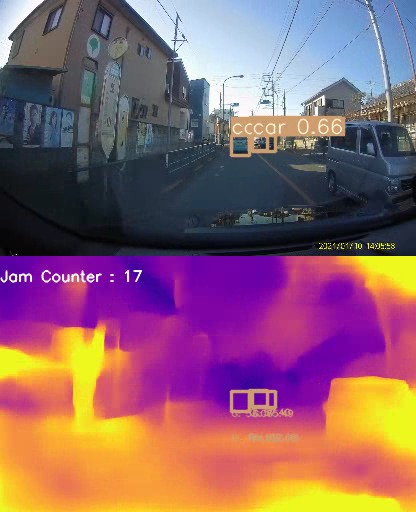
\includegraphics[width=4.5cm]{figs/ex01_01after.png}
    \end{center}
  \caption{結果1}
  \label{fig:ex01_01after}
\end{minipage}

  \begin{minipage}{0.33\hsize}
  \begin{center}
    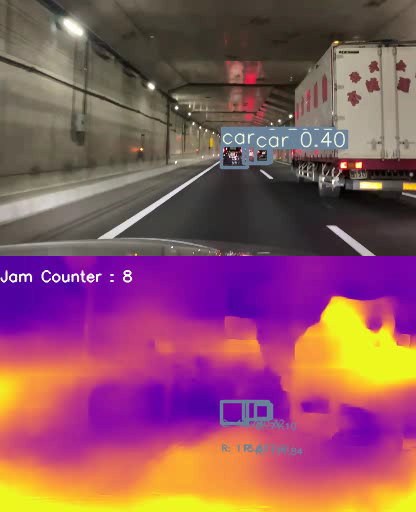
\includegraphics[width=4.5cm]{figs/ex01_02after.png}
  \end{center}
  \caption{結果2}
  \label{fig:ex01_02after}
\end{minipage}

  \begin{minipage}{0.33\hsize}
  \begin{center}
    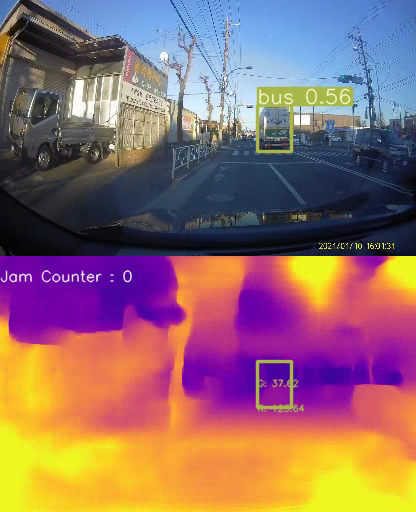
\includegraphics[width=4.5cm]{figs/ex01_03after.png}
  \end{center}
  \caption{結果3}
  \label{fig:ex01_03after}
\end{minipage}
\end{tabular}
\end{figure}
% ---------------------------------------------------

\figref{fig:ex01_01after},\figref{fig:ex01_02after}および\figref{fig:ex01_03after}からわかる通り,左右の1/3を検出しないことで先行車のみを検出し,より正しく渋滞推定を行うことができている.
また,実験1と実験2における動画の中で渋滞だと検出した回数の比較の表を以下に示す.

% ----------------------------------------------------
\begin{table}[htbp]
  \centering
  \begin{scriptsize}
  \begin{tabular}{ccc}
  \toprule
映像番号 & 実験1 & 実験2\\
  \midrule
映像1 & 425 & 131\\
映像2 & 1309 & 401\\
映像3 & 256 & 59\\
映像4 & 1364 & 65\\
  \bottomrule
  \end{tabular}
  \end{scriptsize}
  \caption{実験2 - 結果}
  \label{tab:dataset}
\end{table}
% ------------------------------------------------------

\section{まとめ}
本章では,本研究におけるシステムの実装とシステム改良のための予備実験について述べた.
予備実験では使用する深度推定ライブラリの決定,画像圧縮問題の解決および評価基準の決定を行った.
次章では本研究における本実験について述べる.